\chapter{Исследование многозадачного обучения}\label{ch:ch5}

В этой главе рассматривается использование методов дообучения и многозадачного обучения для получения модели, способной одновременно осваивать несколько навыков рассуждения, представленных в BABILong. Экспериментально показывается, что модели с числом параметров менее 140 миллионов могут превосходить значительно большие аналоги за счёт эффективного освоения нескольких ключевых задач одновременно. Добавление условия перед началом контекста в модель Recurrent Memory Transformer позволяет достичь наилучших результатов на подмножестве задач QA1-QA5 из BABILong для контекстов длиной до 32k токенов. Более того, модель демонстрирует способность к обобщению на новые задачи и увеличенные длины входных данных, а также обладает большей устойчивостью к изменениям во входной информации.

\section{Многозадачное обучение и тестирование}

Целью данной части работы является обучение единой модели, способной одновременно решать несколько задач из BABILong, вместо использования отдельных моделей для каждой из них. Эффективность такого подхода демонстрируется с использованием Recurrent Memory Transformer с всего 137 миллионами параметров, основанного на GPT-2. Дополнительно анализируется влияние многозадачного обучения и взаимный эффект от обучения на задачах из BABILong.

Также предлагается подход к улучшению многозадачного обучения в RMT (Recurrent Memory Transformer) за счёт оптимальной организации данных: размещение вопроса в начале текста увеличивает среднюю точность на 12\% и улучшает качество решения отдельных задач. Данный метод позволяет добиться лучших результатов на задачах QA1–QA5 из BABILong, превосходя GPT-4 и другие модели при обработке контекстов длиной до 32k токенов. Также анализируется взаимный эффект от обучения на различных задачах и способность модели к обобщению на новые задачи и длины контекста, демонстрируется её устойчивость к изменениям имён и объектов.

Для анализа моделей с длинным контекстом, используется бенчмарк BABILong включающий в себя 20 разнообразных задач. Эти задачи проверяют способности к различным видам мышления, включая связывание фактов, индукцию, дедукцию, подсчет и обработку данных в множествах и списках. Примеры BABILong формируются путем встраивания заданий из набора данных bAbI~\cite{WestonBCM15} в случайные предложения из текстов корпуса PG-19~\cite{rae2019compressive}. Изменяя объем фонового текста, можно регулировать длину задач от исходного уровня в 0 токенов, соответствующего задачам bAbI без дополнительных данных, до 10 миллионов токенов и более.

Задачи BABILong отличаются по уровню сложности и типу рассуждений. Например, QA1 («single supporting fact») требует определения местонахождения человека на основе единственного факта. QA2 и QA3 (two supporting facts» и «three supporting facts») предполагают необходимость различать субъекты и объекты при использовании двух или трёх фактов. QA4 («two-argument relations») направлено на пространственные рассуждения, а QA5 («three-argument relations») требует отслеживания нескольких объектов для решения задачи. Более подробная информация о задачах представлена в работе по bAbI~\cite{WestonBCM15}.

\subsection{Формат входных данных}

Для обучения моделей используется следующий формат ввода, варьируя расположение вопроса — в начале или в конце:

\begin{verbatim} 
    
    1. {Контекст}\n\nВопрос: {Вопрос} 
    
    2. Вопрос: {Вопрос} {Контекст}\n\nВопрос: {Вопрос} 

\end{verbatim}

В предыдущих экспериментах применялся первый вариант, где вопрос располагался в конце. Этот подход более сложен, так как модель сначала анализирует контекст без знания вопроса. Размещение вопроса в начале позволяет использовать знание о задаче при обработке контекста, что может повысить эффективность решения. В текущем исследовании преимущественно используется второй формат. Однако для оценки LLM сохраняется первый формат, дополненный инструкциями, примерами и завершающим запросом.


\subsection{Постановка эксперимента}

Модель RMT обучается на первых десяти задачах (QA1–QA10), а задачи QA11 и далее используются для оценки способности обобщать на новые данные. При обучении задачи выбираются случайным образом для каждого шага обучения. Размер сегментов в RMT составляет 512 токенов, объем памяти ограничен 16 токенами.

Согласно предыдущим исследованиям~\cite{kuratov2024babilong}, используется подход последовательного увеличения числа сегментов в следующем порядке: 1-2-4-6-8-16-32. Обучение завершается на этапе 32 сегментов (16k токенов). На каждом этапе число сегментов варьируется от $1$ до $n$. Скорость обучения выбирается из диапазона {5e-05, 1e-05}, используется оптимизатор AdamW с линейным расписанием изменения скорости и начальным разогревом. Обучение продолжается в течение 5000 либо 10000 шагов с остановкой при отсутствии роста метрик. В основе модели лежит предварительно обученная GPT-2 137M из каталога Hugging Face\footnote{https://huggingface.co/openai-community/gpt2}. Также проводилось дообучение модели Phi-3-mini\footnote{https://huggingface.co/microsoft/Phi-3-mini-128k-instruct} на многозадачном наборе данных с длиной контекста 4096 токенов. Для обучения использовался оптимизатор AdamW, косинусное расписание изменения скорости и разогревом на протяжении 15 эпох. В экспериментах использовались до четырёх GPU Nvidia A100 80GB.

\begin{figure}
    \vskip -0.1in
    \centering
    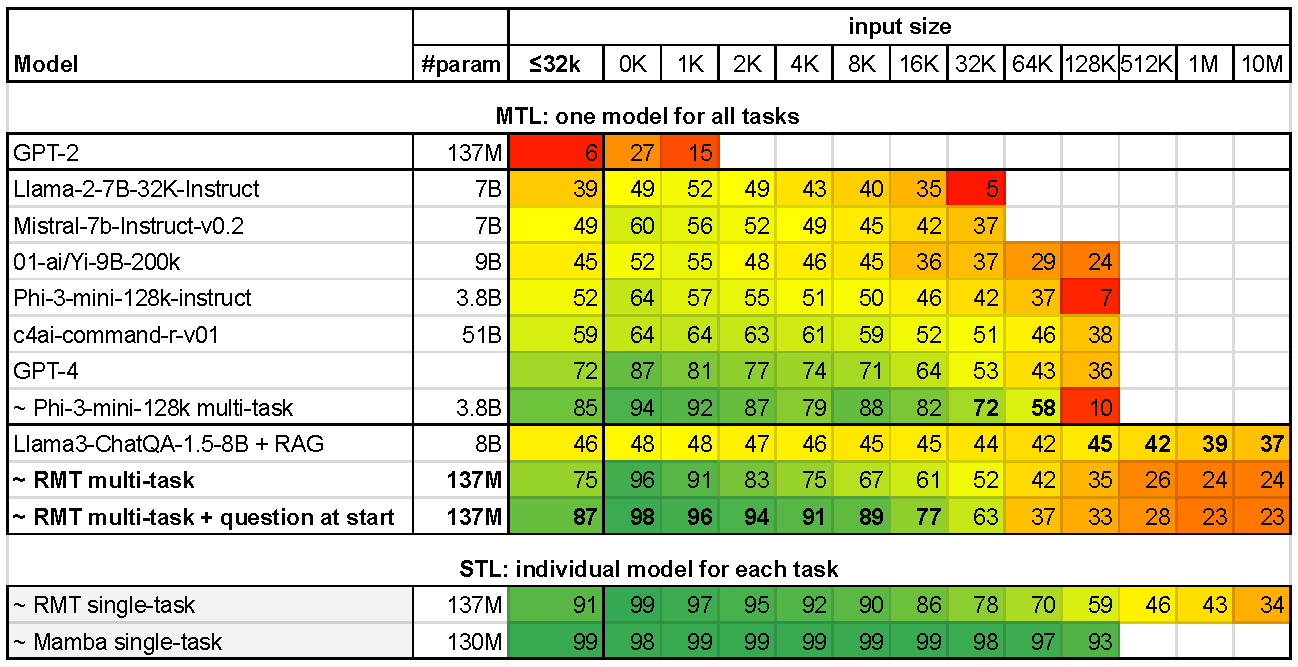
\includegraphics[width=\linewidth]{images/part5/main_table.pdf}
    \caption{Средняя точность решения задач QA1–QA5. RMT, обученная на BABILong, показывает наилучшие результаты в многозадачном режиме при длине задач до 32k токенов. Для более длинных контекстов лидирует Llama-3 с механизмом поиска. Знак \textbf{$\sim$} указывает дообучение на BABILong. STL — обучение на отдельных задачах с разными моделями, MTL — обучение на смеси задач с одной моделью. $\leq32k$ обозначает средний результат для контекстов до 32k токенов.}
    \label{fig:main_table}
    \vskip -0.1in
\end{figure}

На Рисунке~\ref{fig:main_table} показано сравнение языковых моделей на задачах BABILong при обучении на одной задаче (STL) и многозадачном обучении (MTL). Для соответствия условиям оценки из~\cite{kuratov2024babilong}, результаты обученных моделей сравниваются с большими языковыми моделями (LLM) на первых пяти задачах. Модели RMT и Mamba в нижней части таблицы были дообучены в режиме STL, где каждая задача обучалась на отдельной модели, а результаты усреднялись. В верхней части представлены результаты, полученные с использованием одной модели для всех пяти задач, что делает задачу более сложной, что видно из различий в оценках RMT.

Дообучение Phi-3-mini демонстрирует значительное увеличение средней точности, превышающее 30\%. Однако модель испытывает значительное снижение качества при увеличении размера контекста до 128k токенов. Несмотря на сложность MTL-конфигурации, многозадачный RMT достигает лушчих результатов для длины последовательностей до 32k токенов, превосходя LLM, параметры которых превышают его более чем в 100 раз. Повторение вопросов в начале входных данных увеличивает точность в среднем на 12\%. Тем не менее, качеством многозадачной модели RMT деградирует с ростом размера контекста быстрее, чем в режиме STL.

\subsection{Анализ способности к обобщению}

Для изучения эффективности многозадачного обучения RMT анализируется, как обучение на одной задаче влияет на результаты на других и дает ли многозадачное обучение преимущества перед однозадачным. Для экспериментов используются версии задач BABILong с коротким контекстом (512 токенов), что упрощает задачу за счет устранения необходимости фильтрации данных из больших объемов текста и сосредотачивает внимание на сути задач.
\subsection{Влияние размера обучающей выборки}

Результаты показывают, что RMT, обученный на 10 задачах, превосходит большие языковые модели. Возникает вопрос: какое минимальное количество задач нужно для достижения аналогичных результатов? Для ответа размер обучающей выборки последовательно увеличивается, и оцениваются средние результаты по QA1-QA10. QA11-QA15 исключены из обучения для проверки обобщающей способности.

Как показано на Рисунке~\ref{fig:number_of_tasks}, увеличение числа задач способствует росту качества решения. Наиболее заметное улучшение дает добавление QA3 и QA6, в отличие от QA2 и QA4. После шести задач рост качества стабилизируется, дальнейший прирост минимален. Обучение на шести задачах позволяет превзойти Phi-3-mini, а восьми — GPT-4.

Результаты на задачах вне обучающей выборки (Рисунок~\ref{fig:number_of_tasks}, справа) показывают прирост на 10\% при обучении на всех 10 задачах. Возможности обобщения ограничены размерами GPT-2, но RMT в MTL-режиме заметно превосходит однозадачные модели, демонстрируя важность многозадачного подхода.

\begin{figure}
    \centering
    \vskip -0.1in
    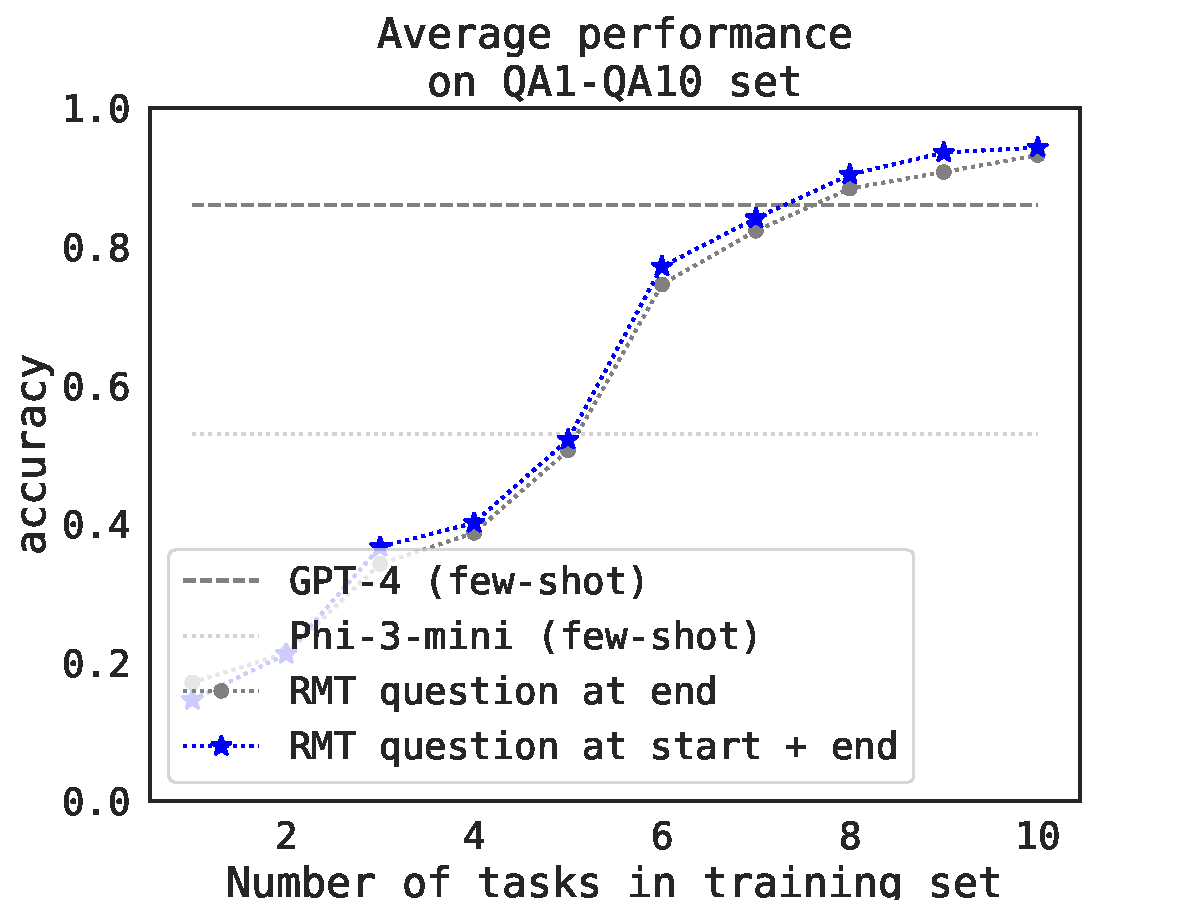
\includegraphics[width=0.49\linewidth]{images/part5/count_tasks_in_domain_v2.pdf}
    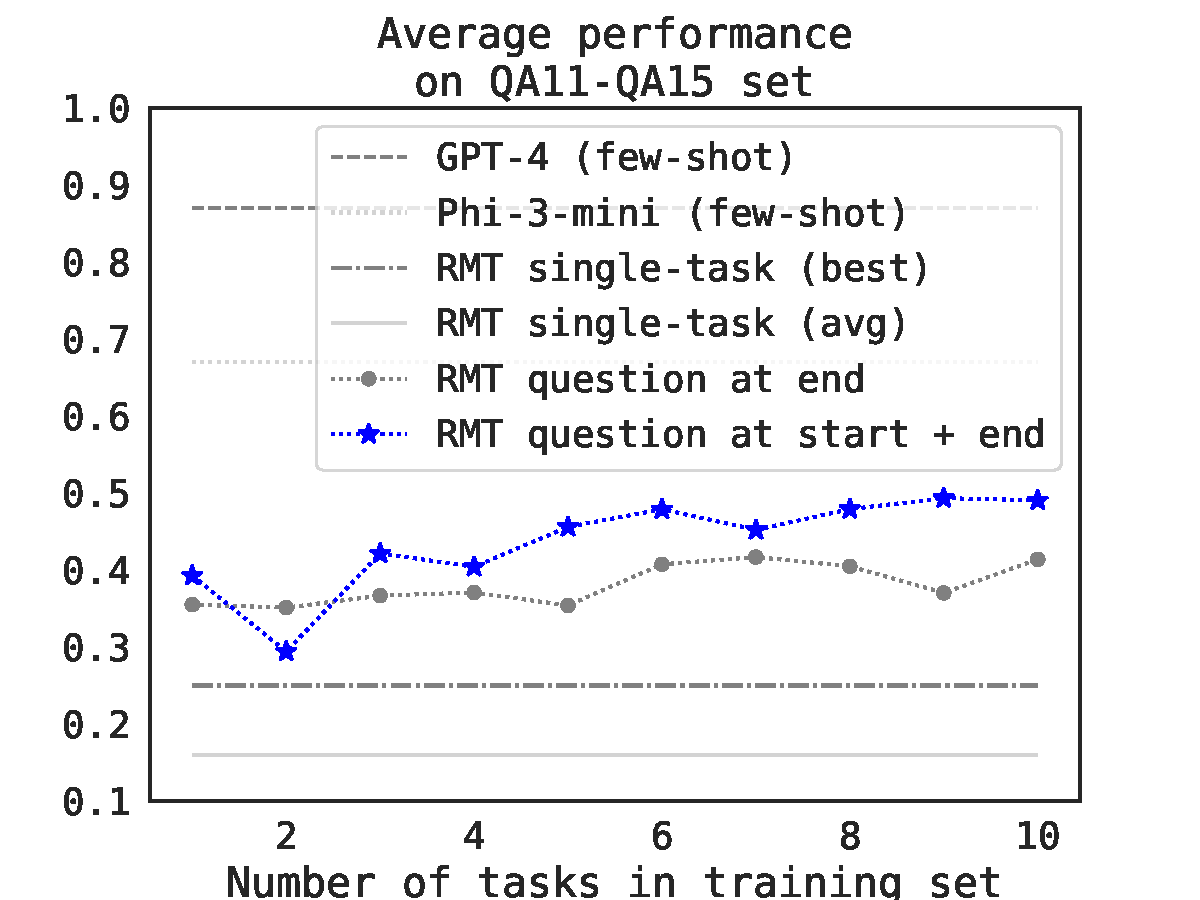
\includegraphics[width=0.49\linewidth]{images/part5/count_tasks_out_of_domain_v2.pdf}
    \caption{Расширение набора задач в обучающем датасете RMT способствует улучшению результатов на задачах из обучающей выборки QA1-QA10 \textbf{(слева)} и повышает способность к обобщению на новые задачи QA11-QA15 \textbf{(справа)}. Каждая задача имеет длину 512 токенов, что эквивалентно одному сегменту.}
    \label{fig:number_of_tasks}
    \vskip -0.1in
\end{figure}

Результаты оценки моделей на задачах из обучающей выборки приведены на рисунке~\ref{fig:number_of_tasks} (слева). Как ожидалось, добавление новых задач в обучение способствует стабильному росту качества решения. Наибольший прирост достигается при добавлении задач QA3 и QA6, по сравнению с QA2 и QA4. Однако после включения шести задач результаты выходят на плато, и дальнейшее увеличение количества задач дает лишь незначительные улучшения. Примечательно, что RMT, обученная всего на шести задачах, уже превосходит модель Phi-3-mini, не проходившую обучение на BABILong, а при обучении на восьми задачах она опережает модель GPT-4.

На рисунке~\ref{fig:number_of_tasks} (справа) показано, что качество решения задач вне обучающей выборки увеличивается всего на 10\% при добавлении всех 10 задач. Незначительность прироста объясняется сравнительно небольшой мощностью базовой модели GPT-2. Однако даже в этих условиях RMT, обученная на нескольких задачах одновременно, значительно превосходит модели, работающие с одной задачей, что подтверждает важность многозадачного подхода для улучшения обобщающих способностей.

\subsection{Взаимный эффект от обучения на задачах BABILong}

Важный вопрос заключается в том, насколько навыки, используемые для решения различных задач, связаны между собой. Если навыки пересекаются, обучение на одной задаче может улучшить результаты на другой. Для проверки этого предположения были выбраны семь задач BABILong с одинаковыми метками: 'bathroom', 'bedroom', 'garden', 'hallway', 'kitchen', 'office'. Обучение на задачах с такими метками дает возможность передать знания между ними.

\begin{figure}
    \centering
    \vskip -0.1in
    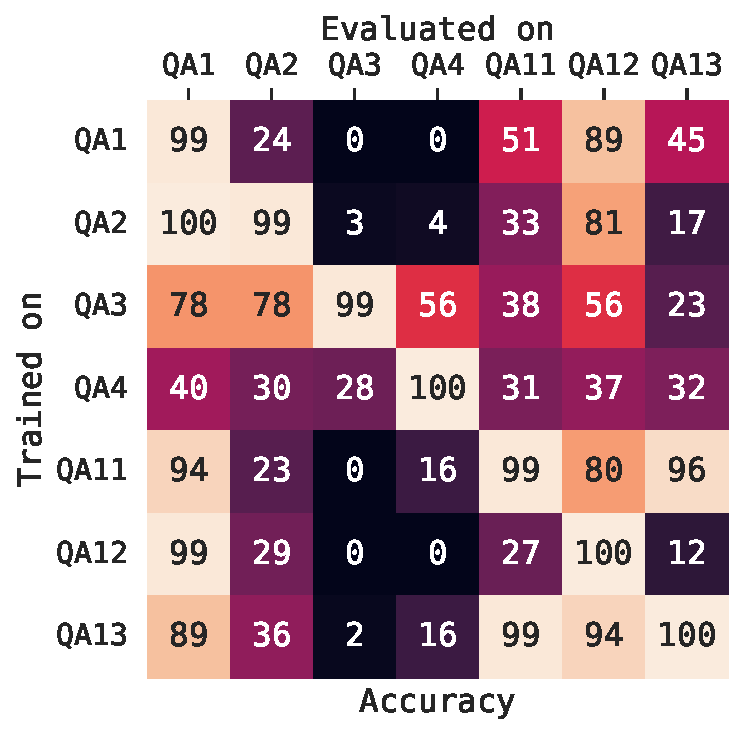
\includegraphics[width=0.45\linewidth]{images/part5/extrapolation_1vs1.pdf}
    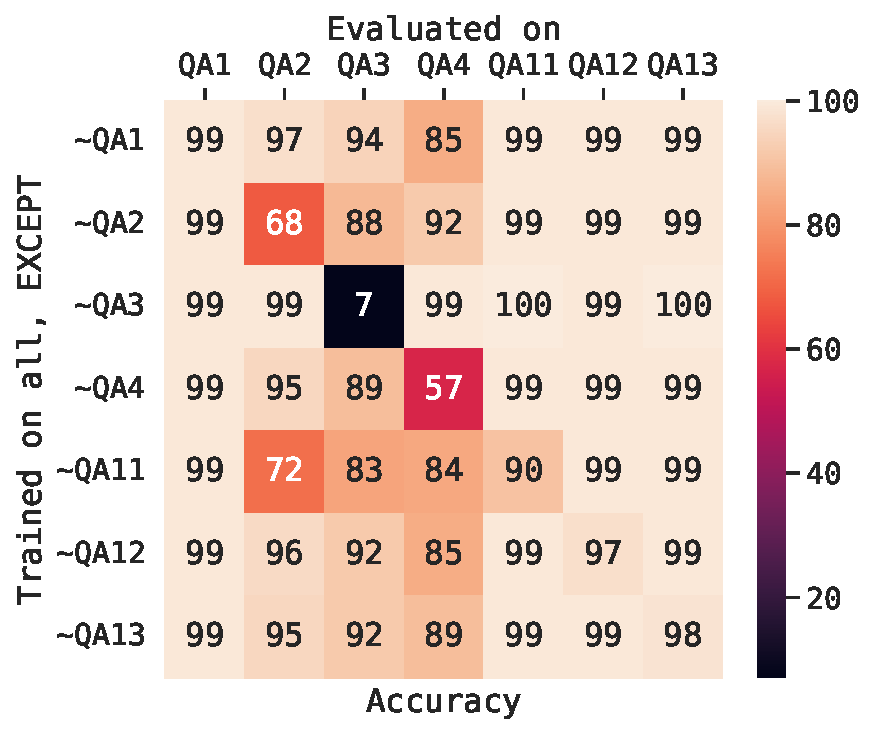
\includegraphics[width=0.54\linewidth]{images/part5/extrapolation_allvs1.pdf}
    \caption{\textbf{Слева}: Обучение на задачах BABILong способствует повышению качества решения задач с той же меткой. \textbf{Справа}: Обучение на задачах с одинаковой меткой позволяет RMT решать выбранную задачу с почти абсолютной точностью. Длина задачи фиксирована на уровне 512 токенов, что эквивалентно одному сегменту.}
    \label{fig:mutual_task_effect}
    \vskip -0.1in
\end{figure}

Изначально обучается отдельную модель для каждой из семи задач и проверяем её работу на оставшихся шести задачах, что представлено на левом графике рисунка~\ref{fig:mutual_task_effect}. Результаты показывают, что такие задачи, как QA1 и QA12, относительно просты и могут быть частично освоены через обучение на других задачах. В отличие от этого, QA3, требующая отслеживания нескольких объектов, и QA4, связанная с пространственными отношениями, могут быть эффективно изучены только через целенаправленное обучение на этих задачах. Также установлено, что QA11 и QA13 оказывают взаимное положительное воздействие друг на друга, в то время как связь между QA12 и QA13 носит асимметричный характер: QA13 способствует освоению QA12, но не наоборот. Более простые задачи, такие как QA1 и QA12, практически не оказывают влияния на более сложные QA3 и QA4.

Эти выводы подтверждаются экспериментом, представленным на правом графике рисунка~\ref{fig:mutual_task_effect}. Здесь модель обучается на шести задачах, за исключением одной, и оценивается на всех семи задачах. Подобно обучению на одной задаче, QA3 и QA4 остаются сложными, даже если модель выучивает все остальные задачи. В то же время задачи QA1, QA12 и QA13 практически полностью выучиваются, даже если они исключены из обучающей выборки. Эти данные демонстрируют сложную и разноплановую структуру задач BABILong, подчёркивая важность освоения нескольких навыков для успешного прохождения всего набора задач.

\subsection{Обобщение на задачи с большей длиной}

Особенностью RMT является способность к обобщению на длины последовательностей, не использовавшиеся при обучении. Однако способна ли модель сохранять эту способность при работе с новыми задачами? Чтобы ответить на этот вопрос, проводится тестирование многозадачной версии RMT, обученной на QA1-QA10, на задачах вне обучающей выборки QA11-QA15. Для сравнения с моделями, обученными в режиме STL, были рассчитаны средние показатели десяти моделей, каждая из которых была обучена на отдельной задаче QA1-QA10, на задачах QA11-QA15 для разных длины последовательностей. Модели RMT обучались на последовательностях длиной до 32 сегментов (16k токенов) и тестировались на последовательностях длиной от 0k до 128k токенов.

\begin{figure}
    \centering
    \vskip -0.1in
    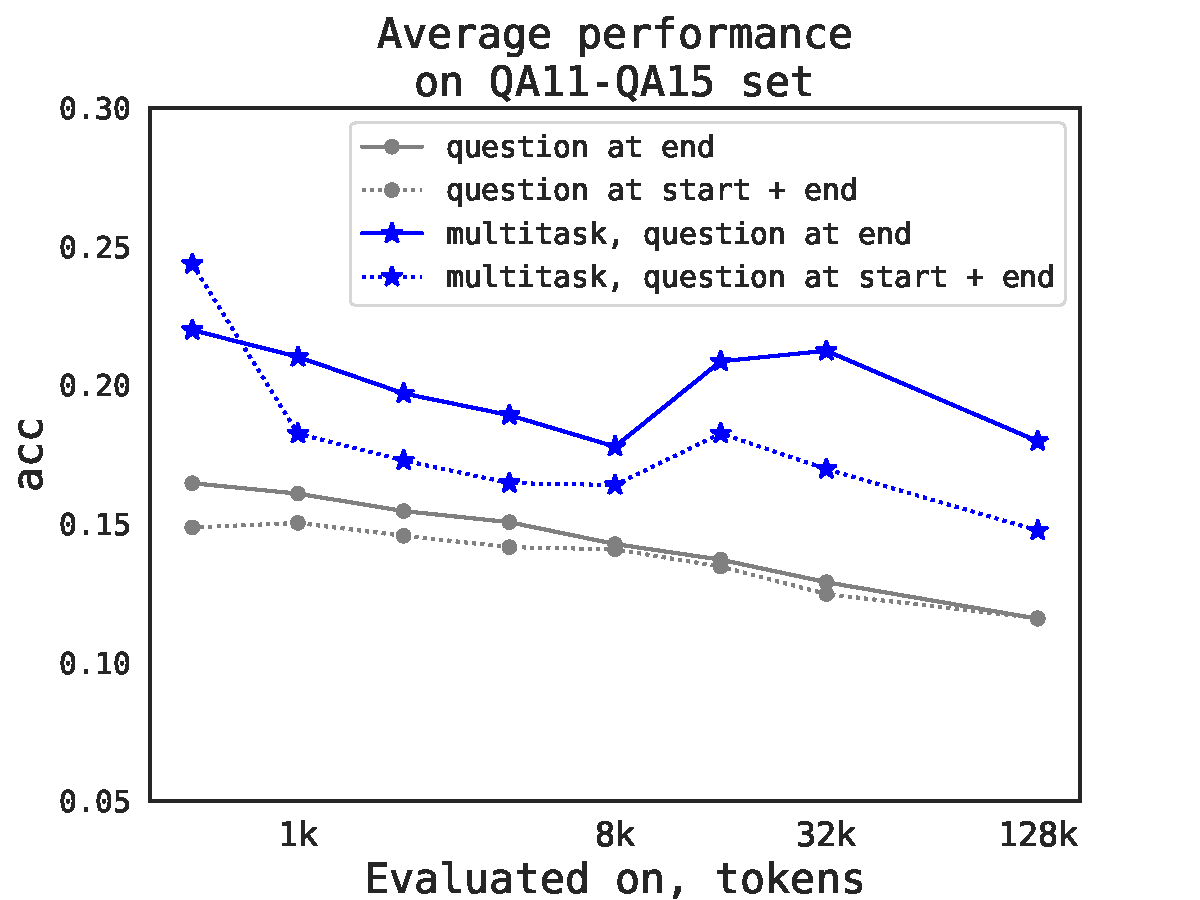
\includegraphics[width=0.65\linewidth]{images/part5/ood_long_context_v2.pdf}
    \caption{Многозадачное обучение улучшает обобщение на новые задачи и большие контексты. RMT, обученный в многозадачном режиме на 32 сегментах QA1-QA10, сравнивается с усредненными значениями качества для однозадачных моделей, обученных на QA1-QA10. Результаты включают конфигурации: с вопросом в конце и с его повторением в начале и конце последовательности. Показатели усреднены по задачам QA11-QA15.}
    \label{fig:ood_long_context}
    \vskip -0.1in
\end{figure}

Результаты показывают, что многозадачная версия RMT значительно превосходит одноцелевые модели, даже при коротких последовательностях, сохраняя это преимущество на более длинных контекстах. Способность модели решать задачи на незнакомых длинах последовательностей подтверждает преимущества многозадачного подхода. На графиках заметны пики на длинах 16k и 32k токенов, вероятно, связанные с переобучением на этих длинах, что улучшает результаты на этих сегментах.

\subsection{Исследование устойчивости}

Было сделано предположение, что многозадачное обучение не только улучшает обобщение, но и повышает устойчивость к изменениям формулировки задач. Для проверки этой гипотезы были изменены имена сущностей (людей, объектов, мест) в пяти задачах (QA1-QA5), при этом метки и связанные сущности во входных данных оставались неизменными. Модели RMT тестировались на последовательностях длиной от 0k до 32k токенов, а результаты усреднялись по задачам, как показано на Рисунке~\ref{fig:robustness}.

\begin{figure}
    \centering
    \vskip -0.1in
    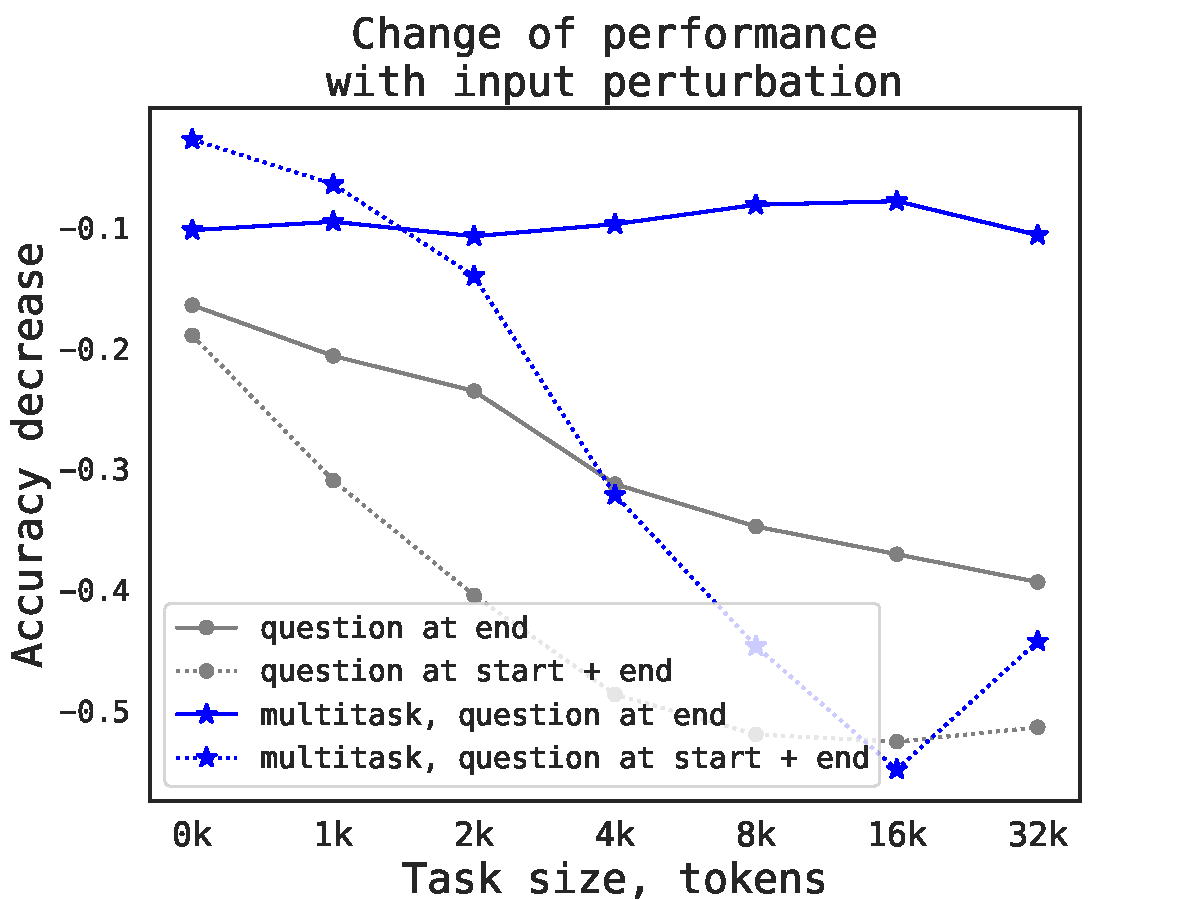
\includegraphics[width=0.65\linewidth]{images/part5/change_task_v2.pdf}
    \caption{Многозадачное обучение улучшает устойчивость RMT к изменениям во входных данных. Качество оценивалось на QA11-QA15 с измененными именами сущностей, и для разных длины последовательностей. Все модели обучались на 32 сегментах; многозадачные версии обучались одновременно на QA1-QA10, а результаты для однозадачных версий представляют усредненное качество моделей, обученных на QA1-QA10.}
    \label{fig:robustness}
    \vskip -0.1in
\end{figure}

Полученные данные подтверждают, что многозадачная версия RMT обладает большей устойчивостью к изменениям во входных данных, сохраняя высокое качество даже на последовательностях длиной до 32k токенов. Интересно, что модель с повторением вопроса в начале и конце работает лучше на коротких последовательностях, но теряет в качестве на более длинных. В то же время размещение вопроса только в конце сводит деградацию при росте длины к минимуму для всех протестированных длины последовательностей. Этот результат можно объяснить тем, что модели с вопросом в начале и конце требуется запоминать вопрос для каждого сегмента, что увеличивает сложность задачи при изменении вопроса и его отличии от обучающего распределения.

\section{Обсуждение и выводы}

Данные результаты подтверждают, что задачи с обработкой длинного контекста представляют серьезные трудности даже для самых современных языковых моделей. Однако дообучение небольших моделей позволило нам значительно улучшить показатели на задачах BABILong. В модели RMT изменение структуры ввода, при котором вопрос помещается в начале, приводит к заметному улучшению результатов в пределах обучающего домена. С другой стороны, размещение вопроса в конце иногда показывает лучшие результаты при оценке на новых задачах и увеличенных размерах контекста. Такой эффект может быть связан с переобучением на варианты вопросов в обучающей выборке, что можно исправить путем повышения разнообразия задач. Кроме того, быстрое снижение качества при увеличении размера ввода может объясняться большим переобучением на количество сегментов в обучающих данных.

Предложенный метод многозадачного обучения стабильно улучшает устойчивость к изменениям ввода и усиливает способность моделей к обобщению на новые задачи и длины контекста. Однако эти улучшения ограничены размером базовой модели и объемом ее памяти. Применение базовых моделей большего размера и увеличение объема памяти, например с использованием механизмов ассоциативной памяти, может привести к дальнейшим улучшениям.

Несмотря на преимущества многозадачного обучения, обучение моделей на одной задаче остается практичным выбором, поскольку оно обеспечивает несколько более высокое качество, если обобщение не требуется. Хотя этот подход ограничен в плане устойчивости и качества работы за пределами обучающего домена, он может быть предпочтительным в ряде случаев. Для повышения результатов многозадачных моделей RMT можно использовать базовые модели с более мощными языковыми возможностями. Однако такие модели RMT демонстрируют более быстрое снижение качества на длинных контекстах по сравнению с однозадачными моделями RMT или конвейером RAG. Одним из решений проблемы переобучения на длину контекста может стать более агрессивный отбор длин на этапе обучения, а также эксперименты с методами поэтапного обучения.

Генерализация моделей RMT на новые задачи остается слабее по сравнению с большими языковыми моделями, особенно для задач с ответами, отсутствующими в обучающей выборке. Основной причиной этого является использование менее мощной базовой модели GPT-2, которая может быть заменена на более сильную. Тем не менее, данные результаты показывают, что дообучение небольших моделей может быть эффективным способом решения сложных задач с длинным контекстом, исключая необходимость в обучении значительно больших моделей или обучении отдельной модели для каждой задачи.